\chapter{Communication}

Different communications are detailed in this chapter, such as particle and 
frontier communications.

\section{Particle communication}

When the particles are moved, due to the interaction with the electric field and 
the magnetic field, their position can exceed the boundaries of the chunk where 
they reside. After updating the position of each particle, the ones that exceed 
the chunk must be translated to the correct one. The process of particle 
communication is done in two stages: first the particles are moved in the X 
dimension, then in the Y. Several steps are required in each stage.

\subsection{Exchange in X}
%TODO Place figure to describe the movement
All chunks in the X dimension reside in one MPI process, so the exchange of 
particles can be done by shared memory. Care must be taken to avoid concurrent 
writes in the same chunk by different tasks. The proposed solution avoids the 
problem by using temporal queues in each chunk. The process can be described in 
the following steps:
%
\begin{enumerate}
\item \texttt{spread\_local\_particles} Out of bound particles in the X 
direction are extracted from the chunk and placed in the correct target queue 
for local exchange.
\item \texttt{collect\_local\_particles} Each chunk looks for particles in the 
queues of other chunks and collects them.
\end{enumerate}
%
Usually only two target queues are required for each chunk, as the particles can 
only move one chunk per iteration. However, in the initial iteration after the 
initialization of the particle positions, they can move to any other chunk, and 
the process is subsequently more computationally expensive.

% TODO:Should we split this details in another section/chapter involving only
% tasks and TAMPI?
Each step can be implemented using tasks with dependencies, in order to exploit 
local parallelism. One task spreads the particles out of the chunk in the 
corresponding queues, so it needs to read and write only the current chunk.
%
\begin{lstlisting}
for (i = 0; i < plasma->nchunks; i++)
{
	chunk = &plasma->chunks[i];
	/* Place each particle outside a chunk in the X dimension, in
	 * the lout list */
	#pragma oss task inout(*chunk) label(spread_local_particles)
	for(is = 0; is < sim->nspecies; is++)
	{
		spread_local_particles(sim, chunk, is, global_exchange);
	}
}
\end{lstlisting}
%
The collecting process can now run in parallel, as there is no chance of 
concurrent writes in the same chunk. However, the task can only run if the 
spread process has finished in the neighbour chunks, as otherwise the queues are 
still being written. The dependencies are placed as \texttt{inout} of all 
involved chunks.
%
\begin{lstlisting}
for (i = 0; i < plasma->nchunks; i++)
{
	chunk = &plasma->chunks[i];
	...

	#pragma oss task inout(*chunk) \
@          inout(*prev_chunk) inout(*next_chunk) \
@          label(collect_local_particles)
	{
		/* Only the two neighbours are needed */
		concat_particles(chunk, prev_chunk);
		concat_particles(chunk, next_chunk);
	}
}
\end{lstlisting}
%
Notice that in the first iteration the collect step must wait for all the spread 
tasks to finish, as the particles can be moved to any block, and thus we expect 
to see a slower iteration than the rest of the simulation.

Once all collecting tasks are completed, all particles are now placed in the 
correct chunk in the X dimension, and only the Y movement is left.

\subsection{Exchange in Y}
%TODO Place figure to describe the movement
Once the particles are placed in the correct chunk in the X dimension, the 
relocation to the correct chunk in the Y dimension involves sending the 
particles to another MPI process. The steps can be resumed as
%
\begin{enumerate}
\item Place each particle out of the chunk bounds in the target queue.
\item Pack the particles to be sent to the neighbour chunk in a message.
\item Send the message in blocks of fixed size.
\item Receive messages from other chunks.
\item Unpack the particle message and place the particles in the chunk.
\end{enumerate}
%
\begin{figure}
\centering
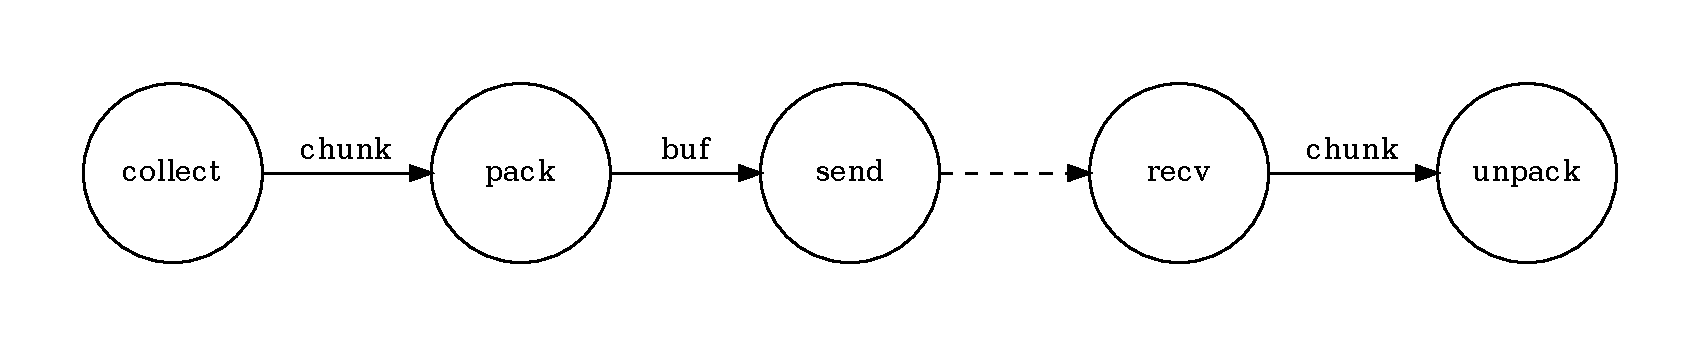
\includegraphics[width=\textwidth]{comm-particles.pdf}
\end{figure}
%
Similarly as for the horizontal direction, the particles exceeding the limits of 
each chunk in the Y dimension are placed in a queue.  Once the particles are 
identified within a chunk, they are packed in a message in a contiguous memory 
region. This buffer is then send using \texttt{MPI\_Send} to the neighbour 
process.

The reception process works in the opposite order: each chunk receives the 
communication of the neighbour chunks in the vertical direction. Once a message 
is received is unpacked and the particles are added to the chunk.

Notice that all the communication is independent of the neighbour chunks in the 
horizontal direction, and can be fully parallelized. Some constraints must be 
added to guarantee that no simultaneous writes occur in the same chunk.
